% !TEX root = _individual/flatland.tex

%%%%%%%%%%%%%%%%%%%%%%%%%%%%%%%%%%%%%%%%%%%%%%%%%%%%%%%%%%%%%%%%%%%%%%%%%%%%%%%%
\chapter{Flatland Geometry}

Flatland geometry is a fictional two-dimensional space where particles are
constrained to the page \cite{Abb1884,Asa2008}. This differs from standard 2-D
geometry, which represents a 3-D problem that is invariant in the $z$ axis,
where particles can travel at different polar angles out of the page. The
constraint of living in the page reduces the phase space of the transport
equation, as the flatland solution is only a function of the azimuthal angle
rather than both azimuthal and polar angles. This reduction in phase space makes 
flatland geometry a computationally less burdensome testing ground for new
methods.

Despite being easier computationally to solve, flatland has a few subtle quirks
that need to be taken into account before implementing a solver in that
geometry. Previous work in flatland \cite{Asa2008,Lar2009c} has shown that the
diffusion coefficient for flatland geometry $\frac{1}{2\sigma}$ is different from
the physical diffusion coefficients $\frac{1}{3\sigma}$, but the correct
formulation for flatland diffusion boundary
conditions have remained an unanswered and indeed unasked question. This
chapter answers that question in addition to providing other insights into this
strange geometry.

%%%%%%%%%%%%%%%%%%%%%%%%%%%%%%%%%%%%%%%%%%%%%%%%%%%%%%%%%%%%%%%%%%%%%%%%%%%%%%%%
\section{Transport in flatland}

Two-dimensional $x$-$y$ geometry represents a three-dimensional problem that is
invariant in the $z$ direction. 

The general-geometry steady-state transport equation with isotropic scattering
and an isotropic source is
\begin{equation}\label{eq:generalTransport}
  \vec{\Omega}\vd \grad \psi + \sigma \psi
  = \frac{\sigma_s}{\omega_0} \int_{\Omega} \psi \ud\Omega + \frac{q}{\omega_0} \,.
\end{equation}

\begin{sidewaystable}[hp]
  \centering
  \renewcommand*{\arraystretch}{1.5}
  \begin{tabular}{rcccccc}
\toprule
   Geometry & $\vec{\Omega}$ & Domain $\Omega$ & $\ud\Omega$
   & $\omega_0 \equiv \int_\Omega \ud\Omega$
   & $\omega_1 \equiv \int_\Omega \abs{\vec{\Omega}\vd\vec{i}} \ud\Omega$
   & $\omega_2 \equiv \int_\Omega (\vec{\Omega}\vd\vec{i})^2 \ud\Omega$
\\ \midrule
   1D & $\mu$ & $-1 \le \mu \le 1$ & $\ud\mu$
   & 2 & 1 & $\frac{2}{3}$
   \\
   2D & $\sqrt{1-\mu^2} \cos \theta \vec{i}
   + \sqrt{1-\mu^2} \sin \theta \vec{j}$
   & $-1 \le \mu \le 1$, $0 \le \theta < 2\pi$ & $\ud\mu \ud \theta$
   & $4\pi$ & $2\pi$ & $\frac{4\pi}{3}$
   \\
   Flatland & $\cos \theta \vec{i} + \sin \theta \vec{j}$
   & $0 \le \theta < 2\pi$ & $\ud \theta$
   & $2\pi$ & $4$ & $\pi$
   \\
   3D & $\mu \vec{i}
   + \sqrt{1-\mu^2} \cos \theta \vec{j}
   + \sqrt{1-\mu^2} \sin \theta \vec{k}$
   & $-1 \le \mu \le 1$, $0 \le \theta < 2\pi$ & $\ud\mu \ud \theta$
   & $4\pi$ & $2\pi$ & $\frac{4\pi}{3}$
\\ \bottomrule
  \end{tabular}
  \caption{Geometry descriptions and identities.}
  \label{tab:geometry}
\end{sidewaystable}

%%%%%%%%%%%%%%%%%%%%%%%%%%%%%%%%%%%%%%%%
\clearpage
\subsection{An insightful comparison problem}

On paper, the problem looks like Fig.~\ref{fig:chordFlatland}, where $\theta$
is the azimuthal angle in both flatland and 2-D geometry. However, in flatland,
the line of length $s$ is constrained to the plane, where in 2D, $s$ is the
length of the distance projected onto the plane. The line actually 
\begin{figure}[htb]
  \centering
  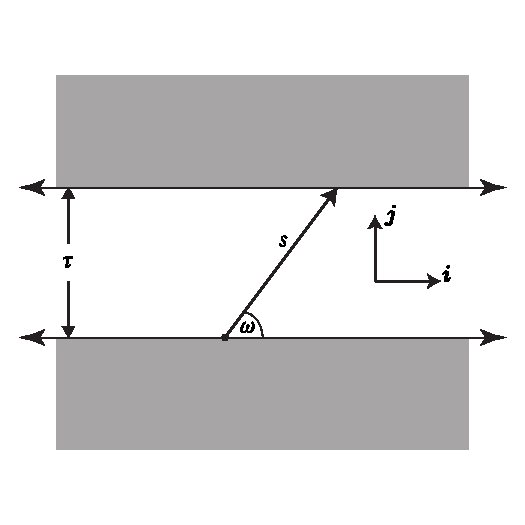
\includegraphics{chord-flatland}
  \caption[The chord length problem as represented on paper.]%
  {The chord length problem as represented on paper. The gap is
  $\tau$ mean free paths apart, $\theta$ is the azimuthal angle, and $s$ is the
  distance across the gap.}
  \label{fig:chordFlatland}
\end{figure}

\begin{figure}[htb]
  \centering
  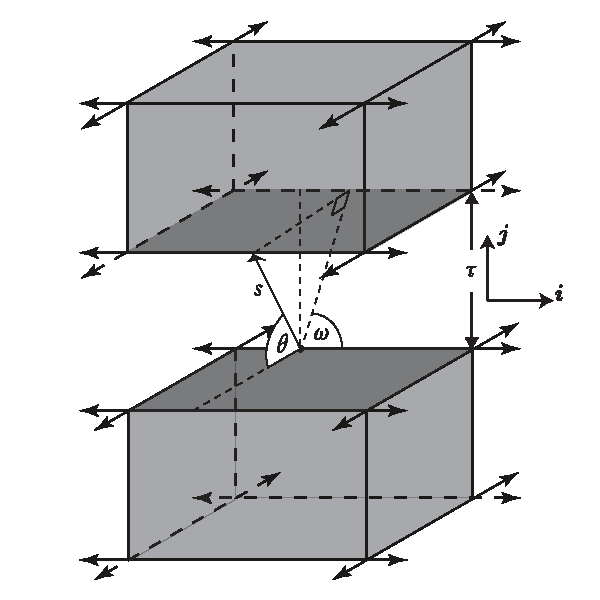
\includegraphics{chord-xyz}
  \caption[A more full view of the chord length problem in 2-D geometry.]%
  {A more full view of the chord length problem in 2-D geometry.
  The polar angle cosine is $\mu= \cos \varphi$, and the azimuthal angle is
  $\theta$.}
  \label{fig:chordFlatland}
\end{figure}

\begin{figure}[htb]
  \centering
  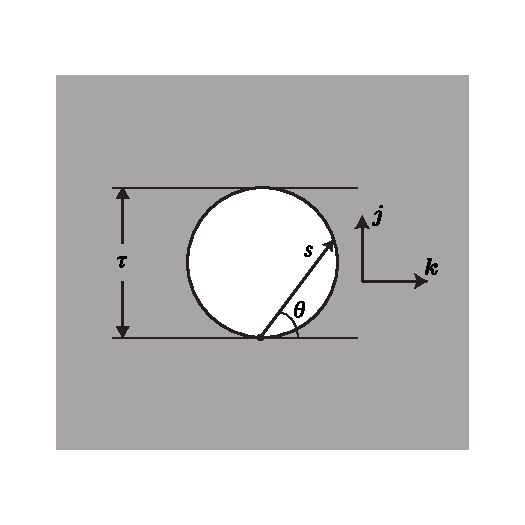
\includegraphics{chord-rz}
  \caption[A cross-section of the chord length problem in $r$--$z$
  geometry.]%
  {A cross-section of the chord length problem in $r$--$z$
  geometry. The orthogonal view looks like Fig.~\ref{fig:chordFlatland}.}
  \label{fig:chordRz}
\end{figure}

Flatland probability of reaching other side:
\begin{equation*}
  p(\tau) = \frac{\int_{0}^{\pi} \eexp^{-\tau / \sin \theta} \sin \theta \ud
  \theta}{\int_{0}^{\pi} \sin \theta \ud \theta}
  = \frac{1}{2} \int_{0}^{\pi} \eexp^{-\tau / \sin \theta} \sin \theta \ud
  \theta
\end{equation*}

2-D probability of reaching other side:
\begin{equation*}
  p(\tau) = \frac{\int_{0}^{\pi} \int_{-1}^{1} \eexp^{-\tau / \left(
  \sqrt{1-\mu^2} \sin\theta \right)}
  \sqrt{1-\mu^2} \sin\theta \ud\mu \ud \theta}
  {\int_{0}^{\pi} \int_{-1}^{1} \sqrt{1-\mu^2} \sin\theta \ud\mu \ud\theta}
  = \frac{\int_{0}^{2\pi} \int_{0}^{1} \eexp^{-\tau / \mu} \mu
  \ud\mu \ud\theta }
  {\int_{0}^{2\pi} \int_{0}^{1} \mu \ud\mu \ud\theta}
  = 2 \int_{0}^{1} \eexp^{-\tau / \mu} \mu
  \ud\mu
\end{equation*}

Cylindrical probability of reaching other side:
\begin{equation*}
  p(\tau) = \frac{\int_{0}^{\pi} \int_{-1}^{1} \eexp^{-\tau \sin \theta / 
  \sqrt{1-\mu^2}}
  \sqrt{1-\mu^2} \sin\theta \ud\mu \ud \theta}
  {\int_{0}^{\pi} \int_{-1}^{1} \sqrt{1-\mu^2} \sin\theta \ud\mu \ud\theta}
  = \frac{1}{\pi} \int_{0}^{\pi} \int_{-1}^{1} \eexp^{-\tau \sin \theta / 
  \sqrt{1-\mu^2}}
  \sqrt{1-\mu^2} \sin\theta \ud\mu \ud \theta
\end{equation*}

\begin{table}[htb]
  \centering
  \begin{tabular}{llll}
\toprule
\phantom{10}$\tau$ & $r$--$z$ & Flatland & $x$--$y$
\\ \midrule
           0.01 & 0.990 & 0.985 & 0.981 \\
\phantom{1}0.1 & 0.906 & 0.863 & 0.833 \\
\phantom{1}1 & 0.404 & 0.274 & 0.219 \\
\phantom{1}10 & 0.00772 & 1.63\EE{-5} & 7.10\EE{-6}
 \\
\bottomrule
  \end{tabular}
  \caption{Comparison of the probability of crossing a channel $\tau$ mfp thick
  without colliding.}
  \label{tab:collision}
\end{table}

%%%%%%%%%%%%%%%%%%%%%%%%%%%%%%%%%%%%%%%%
\clearpage
\subsection{Monte Carlo sampling}
\cite{Lew1984,Bro2004a}
Direct sampling 
probability distribution function (PDF)
cumulative distribution function (CDF)

\subsubsection{Isotropic volume source}
An isotropic internal source, whether directly from an extraneous radiation
source or indirectly from isotropic scattering, has an equal probability of
entering any angle. The normalized  that
represents this process is
\begin{equation*}
  f(\theta) \ud \theta = \frac{1}{2\pi} \ud \theta\,, \quad \theta \in [0, 2\pi)\,.
\end{equation*}
To sample the angle that results from an isotropic event, we use the :
\begin{equation*}
  J(\theta) = \int_{0}^{\theta} f(\theta') \ud \theta' = \frac{1}{2\pi}
  \theta\,.
\end{equation*}
Setting $\xi_1 = J(\theta)$ and solving for $\theta = J\inv(\xi_1)$ gives the
simple result that
\begin{equation*}
  \theta = 2\pi \xi_1\,.
\end{equation*}
The particle's new angle is therefore
\begin{equation*}
  \vec{\Omega} = \cos \theta \vec{i} + \sin \theta \vec{j}
  = \cos 2\pi\xi_1\vec{i} + \sin 2\pi\xi_1 \vec{j}\,.
\end{equation*}

\subsubsection{Isotropic surface source}
Particles emitted from an isotropic surface source have a cosine distribution
\cite{Gre2002}, which makes constant the current in each differential
angle:
\begin{equation}\label{eq:surfaceSource}
  f(\vec{\Omega}) \ud \Omega = c \abs{\vec{\Omega}\vd \vec{n}} \ud \Omega \,,
\vec{\Omega}\vd \vec{n} < 0 \,,
\end{equation}
where $c$ is a normalization constant.

In 3D, with $\vec{n}=\vec{i}$ so $\abs{\vec{\Omega}\vd \vec{n}}=\mu$, this has
the form
\begin{equation*}
  f(\mu, \theta) \ud\mu \ud\theta = \frac{\mu \ud\mu}{2} \frac{\ud\theta}{2\pi}
  \,,\quad 0 \le \mu < 1\,,\ 0 \le \theta < 2\pi\,,
\end{equation*}
a separable distribution that gives $\mu=\sqrt{\xi_1}$ and $\theta=2\pi \xi_2$.

For flatland geometry, the representation is different. Let us choose
$\vec{n} = -\vec{j}$ so that incident directions are inside
$\theta \in [0, \pi)$.
Applying the flatland identities in Table~\ref{tab:geometry} to
Eq.~\eqref{eq:surfaceSource} gives
\begin{equation*}
  f(\theta) \ud\theta = c\abs{ -\sin \theta}
  = c \sin \theta \,,\quad 0 \le \theta < \pi\,.
\end{equation*}
Integrating this gives
\begin{equation*}
  J(\theta) \ud\theta = c \left( 1-\cos\theta \right)
  \,,\quad 0 \le \theta < \pi\,,
\end{equation*}
The constant $c$ should satisfy $J(\pi)=1$:
\begin{equation*}
  1 = c (1 - (-1) ) \lra c=\frac{1}{2}\,.
\end{equation*}

Thus, the CDF for particle emission from a surface source in flatland geometry
is
\begin{equation*}
  J(\theta) \ud\theta = \frac{1}{2} \left( 1-\cos\theta \right)
  \,,\quad 0 \le \theta < \pi\,.
\end{equation*}
Solving for $\theta = J\inv(\xi_1)$ gives a sampled angle for a surface source
in flatland:
\begin{equation*}
  \theta = \cos\inv(1 - 2\xi_1)\,.
\end{equation*}
Using the identity $\cos^2 \theta + \sin^2 \theta = 1$, the particle's new angle is
\begin{align*}
  \vec{\Omega} &= \cos \theta \vec{i} + \sin \theta \vec{j} \\
  &=  \cos[ \cos\inv(1 - 2\xi_1) ] \vec{i} + \sin[ \cos\inv(1 - 2\xi_1) ] \vec{j} \\
  &= (1 - 2\xi_1) \vec{i} + \sqrt{1 - (1 - 2\xi_1)^2} \vec{j}\,.
\end{align*}

%%%%%%%%%%%%%%%%%%%%%%%%%%%%%%%%%%%%%%%%%%%%%%%%%%%%%%%%%%%%%%%%%%%%%%%%%%%%%%%%
\section{Diffusion in flatland}

In 2-D geometry, particles diffuse in three dimensions, although their density
is projected onto the 2-D plane. In contrast, flatland particles have one fewer
dimension into which to leak: as we will see, the result is a larger diffusion
coefficient.

The differences in the identities shown in Table~\ref{tab:geometry} result not
only in a different diffusion coefficient but also different boundary
conditions. In this section, we derive boundary conditions from a steady-state
transport equation with isotropic scattering. There is no loss of generality in
ignoring the time dependence because of the quasi-static approximation made in
the derivation of the diffusion coefficient (see \S\ref{sec:diffusion}).

To aid the reader in understanding whence the different coefficients in the
diffusion equation arise, we use the geometric constants given in
Table~\ref{tab:geometry}:
\begin{equation*}
  \omega_n \equiv \int_\Omega \abs{\vec{\Omega} \vd \vec{i}}^n \ud \Omega\,,
\end{equation*}
where $\Omega$ is the domain of the angular variable $\vec{\Omega}$. In 2-D,
$\vec{\Omega}$ sweeps the $4\pi$ unit sphere and is projected to the plane, but
in flatland, $\vec{\Omega}$ lives on a $2\pi$ unit circle.

%%%%%%%%%%%%%%%%%%%%%%%%%%%%%%%%%%%%%%%%
\subsection{Interior diffusion approximation}
The steady-state transport equation with isotropic scattering is
\begin{subequations} \label{eqs:ssTransport}
\begin{equation}\label{eq:ssTransportVol}
  \vec{\Omega}\vd \grad \psi(\vec{x}, \vec{\Omega})
  + \sigma(\vec{x}) \psi(\vec{x}, \vec{\Omega})
  = \frac{1}{\omega_0} \phi(\vec{x}) \,,
  \quad \vec{x} \in V \,,\ \vec{\Omega} \in \Omega\,.
\end{equation}
Here, the scalar angular flux is $\int_{\Omega} \psi \ud \Omega$, and the quantities
$\omega_0$ and $\Omega$ are defined in Table~\ref{tab:geometry}: in flatland,
$\omega_0=2\pi$; in 2D, $\omega_0=4\pi$. We consider a specified incident
boundary condition:
\begin{equation} \label{eq:ssBndy}
  \psi(\vec{x}, \vec{\Omega}) = \psi^b(\vec{x}, \vec{\Omega})
  \quad \vec{x} \in \partial V \,,\ \vec{\Omega} \vd \vec{n} < 0\,.
\end{equation}
\end{subequations}

The diffusion approximation begins by assuming that $\psi$ is linear in angle:
\begin{equation*}
  \psi(\vec{x}, \vec{\Omega}) \approx f(\vec{x}) + \vec{\Omega} \vd
  \vec{g}(\vec{x})\,.
\end{equation*}
The zeroth angular moment of $\psi$ determines $f$:
\begin{equation*}
  \phi = \int_\Omega \psi \ud \Omega
= \int_\Omega \left( f + \vec{\Omega}\vd \vec{g} \right) \ud\Omega
= \int_\Omega\ud\Omega f + 0
= \omega_0 f \,,
\end{equation*}
so $f = \phi/\omega_0$. Similarly, the first moment of $\psi$ gives $g$:
\begin{equation*}
  \vec{J} = \int_\Omega \vec{\Omega} \psi \ud \Omega
= f \int_\Omega \vec{\Omega} \ud\Omega
  + \vec{g} \vd \int_\Omega \vec{\Omega}\vec{\Omega} \ud\Omega
= \omega_2 \vec{g} \,,
\end{equation*}
so $\vec{g} = \vec{J}/\omega_2$. This is the \Pone\ approximation for $\psi$ in the different geometries:
\begin{equation}\label{eq:ssPone}
  \psi(\vec{x}, \vec{\Omega})
  \approx \frac{1}{\omega_0} \phi(\vec{x})
  + \frac{1}{\omega_2} \vec{\Omega} \vd \vec{J}(\vec{x})\,.
\end{equation}

The diffusion approximation is a closure for the first angular moment of
the transport equation, so we now operate on Eq.~\eqref{eq:ssTransportVol} with
$\int_\Omega \vec{\Omega} (\cdot) \ud \Omega$ and substitute
Eq.~\eqref{eq:ssPone}:
\begin{align*}
  \grad \vd \int_\Omega \vec{\Omega} \vec{\Omega} \psi
  \ud\Omega
  + \sigma \int_\Omega \vec{\Omega} \psi \ud\Omega
  &= \frac{1}{\omega_0} \phi(\vec{x}) \int_\Omega \vec{\Omega} \ud\Omega
  \\
  \grad \vd \int_\Omega \vec{\Omega} \vec{\Omega} \psi(\vec{x}, \vec{\Omega})
  \ud\Omega
  + \sigma \vec{J}
  &= 0
  \\
  \grad \vd \int_\Omega \vec{\Omega} \vec{\Omega} \left(
  \frac{1}{\omega_0}\phi + \frac{1}{\omega_2} \vec{\Omega} \vd \vec{J}
  \right) \ud\Omega
  + \sigma \vec{J}
  &= 0
  \\
  \frac{1}{\omega_0} \grad \vd \int_\Omega \vec{\Omega} \vec{\Omega}
  \ud\Omega \phi 
  + \sigma \vec{J} &= 0
  \\
  \frac{\omega_2}{\omega_0} \grad \phi + \sigma \vec{J} &= 0 \,.
\end{align*}
Solving for $\vec{J}$ gives Fick's law, expressed in the general-geometry form:
\begin{equation} \label{eq:fickGeneral}
  \vec{J}(\vec{x})
  = - \frac{\omega_2}{\omega_0} \frac{1}{\sigma(\vec{x})} \grad \phi(\vec{x})
  \equiv -D(\vec{x}) \grad \phi(\vec{x})\,.
\end{equation}
In 2-D and 3-D, $\omega_2/\omega_0 = (4\pi / 3) / (4\pi) = 1/3$; however, in
flatland, $\omega_2/\omega_0 = \pi / (2\pi) = 1/2$. Thus, $D=(3\sigma)\inv$ in
2-D but $D=(2\sigma)\inv$ in flatland.

Substituting Fick's law back into the linear-in-angle approximation,
Eq.~\eqref{eq:ssPone}, we get the diffusion approximation to the angular
angular flux:
\begin{align} \nonumber
  \psi(\vec{x}, \vec{\Omega})
  &\approx \frac{1}{\omega_0} \phi(\vec{x})
  + \frac{1}{\omega_2} \vec{\Omega} \vd \left[ - \frac{\omega_2}{\omega_0}
  \frac{1}{\sigma(\vec{x})} \grad \phi(\vec{x}) \right]\,.
  \\ \label{eq:diffusionIntensity}
  \psi(\vec{x}, \vec{\Omega})
  &= \frac{1}{\omega_0} \left[ \phi(\vec{x})
  - \frac{1}{\sigma(\vec{x})}
  \vec{\Omega} \vd \grad \phi(\vec{x}) \right] \,.
\end{align}
In 2-D, Eq.~\eqref{eq:diffusionIntensity} evaluates to the standard result
\begin{equation*}
 \psi(\vec{x}, \vec{\Omega})
= \frac{1}{4\pi} \left[ \phi(\vec{x}) - \frac{1}{\sigma(\vec{x})} \vec{\Omega}
\vd \grad \phi(\vec{x}) \right] \,,
\end{equation*}
and in flatland, it is
\begin{equation}\label{eq:flatlandDiffusion}
 \psi(\vec{x}, \vec{\Omega})
= \frac{1}{2\pi} \left[ \phi(\vec{x}) - \frac{1}{\sigma(\vec{x})} \vec{\Omega}
\vd \grad \phi(\vec{x}) \right]\,.
\end{equation}

%%%%%%%%%%%%%%%%%%%%%%%%%%%%%%%%%%%%%%%%
\subsection{Marshak boundary condition}
The Marshak boundary condition \cite{Mar1947} preserves the incident radiation
current on the boundary. It is derived by substituting the approximate diffusion
angular flux from Eq.~\eqref{eq:diffusionIntensity} into the boundary condition,
Eq.~\eqref{eq:ssBndy}, multiplying by $\abs{\vec{\Omega}\vd \vec{n}}$, and integrating over
incident directions.
\begin{align*}
\int_{\vec{\Omega}\vd \vec{n} < 0 } \abs{\vec{\Omega}\vd \vec{n}}
\psi^b \ud\Omega
 &= 
\int_{\vec{\Omega}\vd \vec{n} < 0 } \abs{\vec{\Omega}\vd \vec{n}} 
 \frac{1}{\omega_0} \left[ \phi - \frac{1}{\sigma}
  \vec{\Omega} \vd \grad \phi \right]
  \ud\Omega
\\
J^{-}
&= 
\frac{1}{\omega_0} \phi \left( \int_{\vec{\Omega}\vd \vec{n} < 0 }
\abs{\vec{\Omega}\vd \vec{n}} \ud\Omega \right) 
  - \frac{1}{\omega_0}\frac{1}{\sigma}
  \int_{\vec{\Omega}\vd \vec{n} < 0 } (-\vec{\Omega}\vd \vec{n})
  \vec{\Omega} \ud\Omega  \vd \grad \phi
\\
J^{-}
&=
\frac{1}{\omega_0} \phi \left( \frac{\omega_1}{2} \right) 
  + \frac{1}{\omega_0}\frac{1}{\sigma} \vec{n} \vd
  \int_{\vec{\Omega}\vd \vec{n} < 0 } \vec{\Omega} \vec{\Omega} \ud\Omega
  \vd \grad \phi
\\
J^{-}
&=
\frac{\omega_1}{2\omega_0} \phi 
  + \frac{1}{\omega_0}\frac{1}{\sigma} \vec{n} \vd
  \left( \int_{\vec{\Omega}\vd \vec{n} < 0 } \vec{\Omega} \vec{\Omega} \ud\Omega \right)
  \vd \grad \phi
\\
J^{-}
&=
\frac{\omega_1}{2\omega_0} \phi
+ \frac{1}{\omega_0}\frac{1}{\sigma} \vec{n} \vd \left( \frac{\omega_2}{2}
\Identitytens \right) \grad \phi
\\
J^{-}
&=
\frac{\omega_1}{2\omega_0} \phi
+ \frac{\omega_2}{2\omega_0}\frac{1}{\sigma} \vec{n} \vd \grad \phi\,.
\end{align*}
Rearranging gives an expression for the Marshak boundary condition for 
\begin{equation} \label{eq:marshak}
\frac{2\omega_0}{\omega_1} J^{-}
=
\phi + \frac{\omega_2}{\omega_1}\frac{1}{\sigma} \vec{n} \vd \grad \phi
\end{equation}

The value
\begin{equation*}
  z_0 \equiv \frac{\omega_2}{\omega_1}
  =
  \begin{cases}
    \frac{2}{3} \approx 0.6667 & \text{1D, 2D, 3D,} \\
    \frac{\pi}{4} \approx 0.7854 & \text{Flatland,}
  \end{cases}
\end{equation*}
is the Marshak extrapolation distance.

Substituting the diffusion coefficient $D$ from Eq.~\eqref{eq:fickGeneral} gives
\begin{equation*}
\frac{2\omega_0}{\omega_1} J^{-}
= \phi + \frac{\omega_0}{\omega_1} D \vec{n} \vd \grad \phi\,.
\end{equation*}
In 1D, 2D, and 3D, this evaluates to
\begin{equation*}
4 J^{-}
= \phi + 2 D \vec{n} \vd \grad \phi\,,
\end{equation*}
but in flatland it is
\begin{equation*}
\pi J^{-}
= \phi + \frac{\pi}{2} D \vec{n} \vd \grad \phi\,.
\end{equation*}

%%%%%%%%%%%%%%%%%%%%%%%%%%%%%%%%%%%%%%%%
\subsection{Variational boundary condition} \label{sec:varBndy}
It is well known that the Marshak boundary condition is not consistent with the
true transport boundary condition. A lengthy asymptotic boundary layer
matching analysis \cite{Hab1975} shows that the correct weighting of the
boundary condition is not $\abs{\vec{\Omega}\vd\vec{n}}$ but rather
$W(\abs{\vec{\Omega}\vd\vec{n}})$, where $W$ is related to Chandrasekhar's
$H$-function \cite{Cha1960}:
\begin{equation} \label{eq:chandraW}
  W(\mu) = \frac{\sqrt{3}}{2} \mu H(\mu) \,.
\end{equation}
In general geometries, this leads to the extrapolation distance of
\begin{align*}
  z_0 = \frac{\int_{0}^{1} \mu W(\mu) \ud \mu}{\int_{0}^{1} W(\mu) \ud
  \mu} \approx 0.7104\,.
\end{align*}

In real-world geometries, a variational analysis \cite{Mal1991} can be used to
derive a very accurate approximation to $W$:
\begin{equation*}
W(\mu) \approx \mu + \tfrac{3}{2} \mu^2 \,,
\end{equation*}
which gives the approximate extrapolation distance of
\begin{equation*}
  z_0 = \frac{\int_{0}^{1} \mu (\mu + \tfrac{3}{2} \mu^2 ) \ud
  \mu}{\int_{0}^{1} (\mu + \tfrac{3}{2} \mu^2 ) \ud \mu} 
  = \frac{17}{24} \approx 0.7083 \,.
\end{equation*}
%This variational analysis can be imitated by taking a semi-infinite,
%source-free, purely scattering transport problem, assuming the exiting $\psi$ is
%constant in angle, and making a particular demand.

Now we repeat that analysis for flatland rather than real space. The first step
is to consider a homogeneous, purely scattering transport problem in a
semi-infinite plane. The transport equation~\eqref{eq:generalTransport} becomes
\begin{subequations} \label{eqs:flatTransport}
\begin{equation}\label{eq:flatTransportVol}
  \cos \theta \pder{\psi}{x} + \sin \theta \pder{\psi}{y} + \sigma \psi
  = \frac{\sigma}{2\pi} \int_{0}^{2\pi} \psi \ud \theta'\,,\quad
 -\infty < x < \infty,\ 0 \le y < \infty,\ 0 \le \theta < 2\pi\,.
\end{equation}
It has a uniform incident boundary condition,
\begin{equation}\label{eq:flatTransportBndy}
  \psi(x, 0, \theta) = \psi^b(\theta) \,,\quad -\infty < x < \infty,\ 
  0 \le \theta < \pi \,.
\end{equation}
\end{subequations}
Also, because there is no variation in the boundary condition or $\sigma$ along
the $x$ axis, $\tpder{\psi}{x}=0$, and Eq.~\eqref{eq:flatTransportVol} becomes the
one-dimensional transport equation 
\begin{equation*}
  \sin \theta \pder{}{y}\psi(y,\theta) + \sigma \psi(y,\theta)
  = \frac{\sigma}{2\pi} \int_{0}^{2\pi} \psi(y,\theta') \ud \theta'\,.
\end{equation*}
This is \emph{not} the same one-dimensional transport equation as in slab
geometry.

We define the $y$ components of the angular moments of $\psi$ as
\begin{equation} \label{eq:flatPhi}
  \phi_m(y) = \int_{0}^{2\pi} (\vec{\Omega}\vd\vec{j})^m \psi(y,\theta) \ud\theta
  = \int_{0}^{2\pi} (\sin\theta)^m \psi(y,\theta) \ud\theta \,.
\end{equation}

As $y\to\infty$, the angular flux $\psi$ will approach a constant $\varphi/2\pi$,
which gives $\phi_0(\infty)=\varphi$. Concordantly, $\phi_1(\infty)=0$.

Operating on the transport equation with $\int_{0}^{2\pi} (\sin\theta)^m (\cdot)
\ud\theta$ gives the $m$th angular moment in the $y$ direction:
\begin{align} \nonumber
  \pder{}{y} \int_{0}^{2\pi} (\sin\theta)^{m+1} \psi \ud\theta
  + \sigma \int_{0}^{2\pi} (\sin\theta)^{m} \psi \ud\theta
  &= \frac{\sigma}{2\pi} \int_{0}^{2\pi} \psi \ud \theta'
  \int_{0}^{2\pi} (\sin\theta)^{m} \ud\theta
  \\ \label{eq:flatMoments}
  \pder{\phi_{m+1}}{y}
  + \sigma \phi_{m}
  &= \frac{\sigma}{2\pi} \phi_{0}
  \int_{0}^{2\pi} (\sin\theta)^{m} \ud\theta\,.
\end{align}
For $m=0$, the conservation equation, Eq.~\eqref{eq:flatMoments} evaluates to
\begin{equation*}
  \pder{\phi_{1}}{y}
  + \sigma \phi_{0}
  = \frac{\sigma}{2\pi} \phi_{0} (2\pi)
  \lra
  \pder{\phi_{1}}{y} = 0\,.
\end{equation*}
That means the current is a constant, and because $\phi_1(\infty)=0$,
that constant is zero.

Evaluating Eq.~\eqref{eq:flatMoments} for $m=1$ and using the result that
$\phi_{1}=0$, we find
\begin{equation*}
  \pder{\phi_{2}}{y}
  + \sigma \phi_{1}
  = \frac{\sigma}{2\pi} \phi_{0} (0)
  \lra
  \pder{\phi_{2}}{y} = 0\,.
\end{equation*}
Thus $\phi_{2}$ is also a constant. As $y\to\infty$, $\psi\to\varphi/2\pi$, so
\begin{equation*}
  \phi_{2} = \int_{0}^{2\pi} (\sin\theta)^2 \frac{\varphi}{2\pi} \ud\theta
  = \frac{1}{2} \varphi\,.
\end{equation*}
% in 1D, this would be $\int_{-1}^{1}\mu^2\frac{\varphi}{2} \ud \mu =
% \frac{1}{3} \varphi$.

Now, since $\phi_1=0$, we can add $\alpha \phi_1$ to this equation for any
$\alpha$:
\begin{align*}
 \alpha\phi_1 + \phi_{2} &= \frac{\varphi}{2} \\
 \int_{0}^{2\pi} (\alpha \sin\theta + \sin^2\theta)
 \psi(y,\theta) \ud\theta
 &= \frac{\varphi}{2}\,.
\end{align*}
At the boundary $y=0$, $\psi=\psi^b$ for incident angles $0 \le \theta < \pi$. The
variational analysis makes the reasonable approximation that, to leading order,
the exiting particles are isotropically distributed, $\psi(0,\theta)=\psi^\text{out}$.
\begin{equation*}
 \int_{0}^{\pi} (\alpha \sin\theta + \sin^2\theta)
 \psi^b(\theta) \ud\theta
 + \int_{\pi}^{2\pi} (\alpha \sin\theta + \sin^2\theta)\ud\theta \psi^\text{out}
 = \frac{\varphi}{2}\,.
\end{equation*}
The value $\alpha=\pi/4$ eliminates the integral over outgoing directions and
gives a relation between moments of the incident angular flux and the
magnitude of the angular flux as $y\to\infty$:
\begin{equation}\label{eq:varBoundary}
  \int_{0}^{\pi} \left( \frac{\pi}{4} \sin\theta + \sin^2\theta \right)
 \psi^b(\theta) \ud\theta
 = \frac{\varphi}{2}\,.
\end{equation}

Diffusion in flatland approximates the angular flux as 
\begin{equation*}
  \psi(\vec{x}, \vec{\Omega}) \approx \frac{1}{2\pi} \left[ \phi(\vec{x}) -
  \frac{1}{\sigma(\vec{x})} \vec{\Omega}
\vd \grad \phi(\vec{x}) \right]
\end{equation*}
In our simple transport problem, $\vec{\Omega} \vd \grad \phi=\sin\theta
\pder{\phi_0}{y}$. We wish our boundary condition to preserve the value of
$\varphi$ when the diffusion method is used:
\begin{align*}
 \varphi = 2\int_{0}^{\pi} \left( \frac{\pi}{4} \sin\theta + \sin^2\theta \right)
 \psi^b(\theta) \ud\theta
 &= 
  2\int_{0}^{\pi} \left( \frac{\pi}{4} \sin\theta + \sin^2\theta \right)
 \left( \frac{1}{2\pi} \phi -
  \frac{1}{\sigma} \sin\theta \pder{\phi_0}{y}\right)\ud\theta
\\
\int_{0}^{\pi} \left( \frac{\pi}{2} \sin\theta + 2 \sin^2\theta \right)
 \psi^b(\theta) \ud\theta
 &= 
\frac{1}{2\pi} \int_{0}^{\pi} \left( \frac{\pi}{2} \sin\theta + 2 \sin^2\theta
\right)\ud\theta
 \phi -
 \frac{1}{2\pi} \int_{0}^{\pi} \left( \frac{\pi}{2} \sin^2\theta + 2 \sin^3\theta \right)\ud\theta \frac{1}{\sigma} \pder{\phi_0}{y}
  \\
 &= 
 \frac{1}{2\pi} \left( \frac{\pi}{2} [2] + 2 \frac{\pi}{2}
\right) \phi
-
\frac{1}{2\pi} \left( \frac{\pi}{2} \left[ \frac{\pi}{2} \right] + 2 \left[
\frac{4}{3} \right] \right) \frac{1}{\sigma} \pder{\phi_0}{y}
\\
 &= 
  \phi
- \left( \frac{\pi}{8} + \frac{4}{3\pi} \right) \frac{1}{\sigma} \pder{\phi_0}{y}
\,.
\end{align*}
In this problem, we chose a boundary surface normal of $\vec{n}=-\vec{j}$. Now
replacing $\sin \theta$ with $-\vec{\Omega}\vd\vec{n}$, we get the general
boundary condition for flatland diffusion,
\begin{equation} \label{eq:flatlandDiffusionVarBc}
\int_{\vec{\Omega}\vd\vec{n} < 0} \left[ \frac{\pi}{2}
\abs{\vec{\Omega}\vd\vec{n}} + 2 (\vec{\Omega}\vd\vec{n})^2 \right]
\psi^b(\vec{x}, \vec{\Omega}) \ud\Omega
= 
  \phi(\vec{x})
  - \left( \frac{\pi}{8} + \frac{4}{3\pi} \right) \frac{1}{\sigma}
  \vec{n}\vd\grad \phi(\vec{x})\,.
\end{equation}
Essentially, we have shown that the flatland equivalent of the $W$ function,
which we shall call $V$, can be approximated by
\begin{equation}\label{eq:flatlandVariational}
  V(\theta)
  \approx \frac{1}{4}\sin\theta + \frac{1}{\pi} \sin^2\theta \,,\quad
  0 \le \theta < \pi \,,
\end{equation}
which satisfies
\begin{equation*}
  \int_{0}^{\pi} V(\theta) \ud\theta= 1
\end{equation*}
and gives the extrapolation distance
\begin{equation*}
  z = \frac{\int_{0}^{\pi} \sin \theta V(\theta) \ud\theta}{\int_{0}^{\pi}
  V(\theta) \ud\theta} =  \frac{\pi}{8} + \frac{4}{3\pi} \,.
\end{equation*}
% \left( \frac{3\pi^2 + 32}{24\pi} \right)

%%%%%%%%%%%%%%%%%%%%%%%%%%%%%%%%%%%%%%%%%%%%%%%%%%%%%%%%%%%%%%%%%%%%%%%%%%%%%%%%
\clearpage

``Marshak'' extrapolation distance:
\begin{equation*}
  z = \frac{\pi}{4} \approx 0.78540
\end{equation*}
Variational extrapolation distance:
\begin{equation*}
  z = \frac{\pi}{8} + \frac{4}{3\pi} \approx 0.81711
\end{equation*}

%%%%%%%%%%%%%%%%%%%%%%%%%%%%%%%%%%%%%%%%%%%%%%%%%%%%%%%%%%%%%%%%%%%%%%%%%%%%%%%%

